\documentclass[12pt, a4paper]{article}

%%%%%% 	pacotes	%%%%%%%
\usepackage[utf8]{inputenc}
\usepackage[portuguese]{babel}
\usepackage[T1]{fontenc}
%\usepackage{fontspec} % habilita o comando /setmainfont{times new roman}
\usepackage{graphicx, wrapfig} % para importar imagens e para coloca-las ao lado do texto

\usepackage{amsmath, amsfonts, amssymb}

%\usepackage{blindtext} % para gerar textos com o comando \blindtext[1]

\usepackage[left=3cm,right=2cm,top=3cm,bottom=2cm]{geometry} % definindo as medidas das margens do papel

%%%%%%%	preambulo	%%%%%%
%\setmainfont{Times New Roman}
\setlength{\baselineskip}{1.5cm} %define a distancia/espaçamento entre linhas para ser 1.5 cm (o padrao da norma ABNT)
%\setlength{\parindent}{1.25cm} %define o recuo do paragrafo para ser 1.25cm (o padrao da norma ABNT)
\setlength{\parindent}{0cm}

\begin{document}
\pagestyle{empty}

\begin{wrapfigure}{L}{0.1\textwidth} % o parametro L: a posição da imagem em relação ao texto: a esquerda do texto. outros valores: l, r, i, o, R, O, I. Já o segundo parametro indica o quao perto o texto esta da imagem. Mudar apenas o valor numerico
\includegraphics[width=0.065\textheight]{logo ufpe.jpg}
%separando cada linha por multiplos de 1.5cm, o espaçamento padrão segundo as normas da ABNT.

\end{wrapfigure}

\noindent UNIVERSIDADE FEDERAL DE PERNAMBUCO\\CENTRO DE CIÊNCIAS EXATAS E DA NATUREZA\\DEPARTAMENTO DE MATEMÁTICA\\PRINCÍPIOS DE CONTAGEM - 2023.1\\PROFESSOR: WILLIKAT BEZERRA DE MELO\\TURMA: 2Z\\

\begin{flushleft}

MONITOR: JARDEL FELIPE CABRAL DOS SANTOS\\[1cm] 
\end{flushleft}

\begin{center} \textbf{ENCONTRO DE MONITORIA - 25/08/2023\\[1cm]}
\end{center}

\begin{center}
\textbf{PROBLEMAS}
\end{center}


\textbf{1. No grafo \(G\) da figura abaixo:} 

\begin{center}
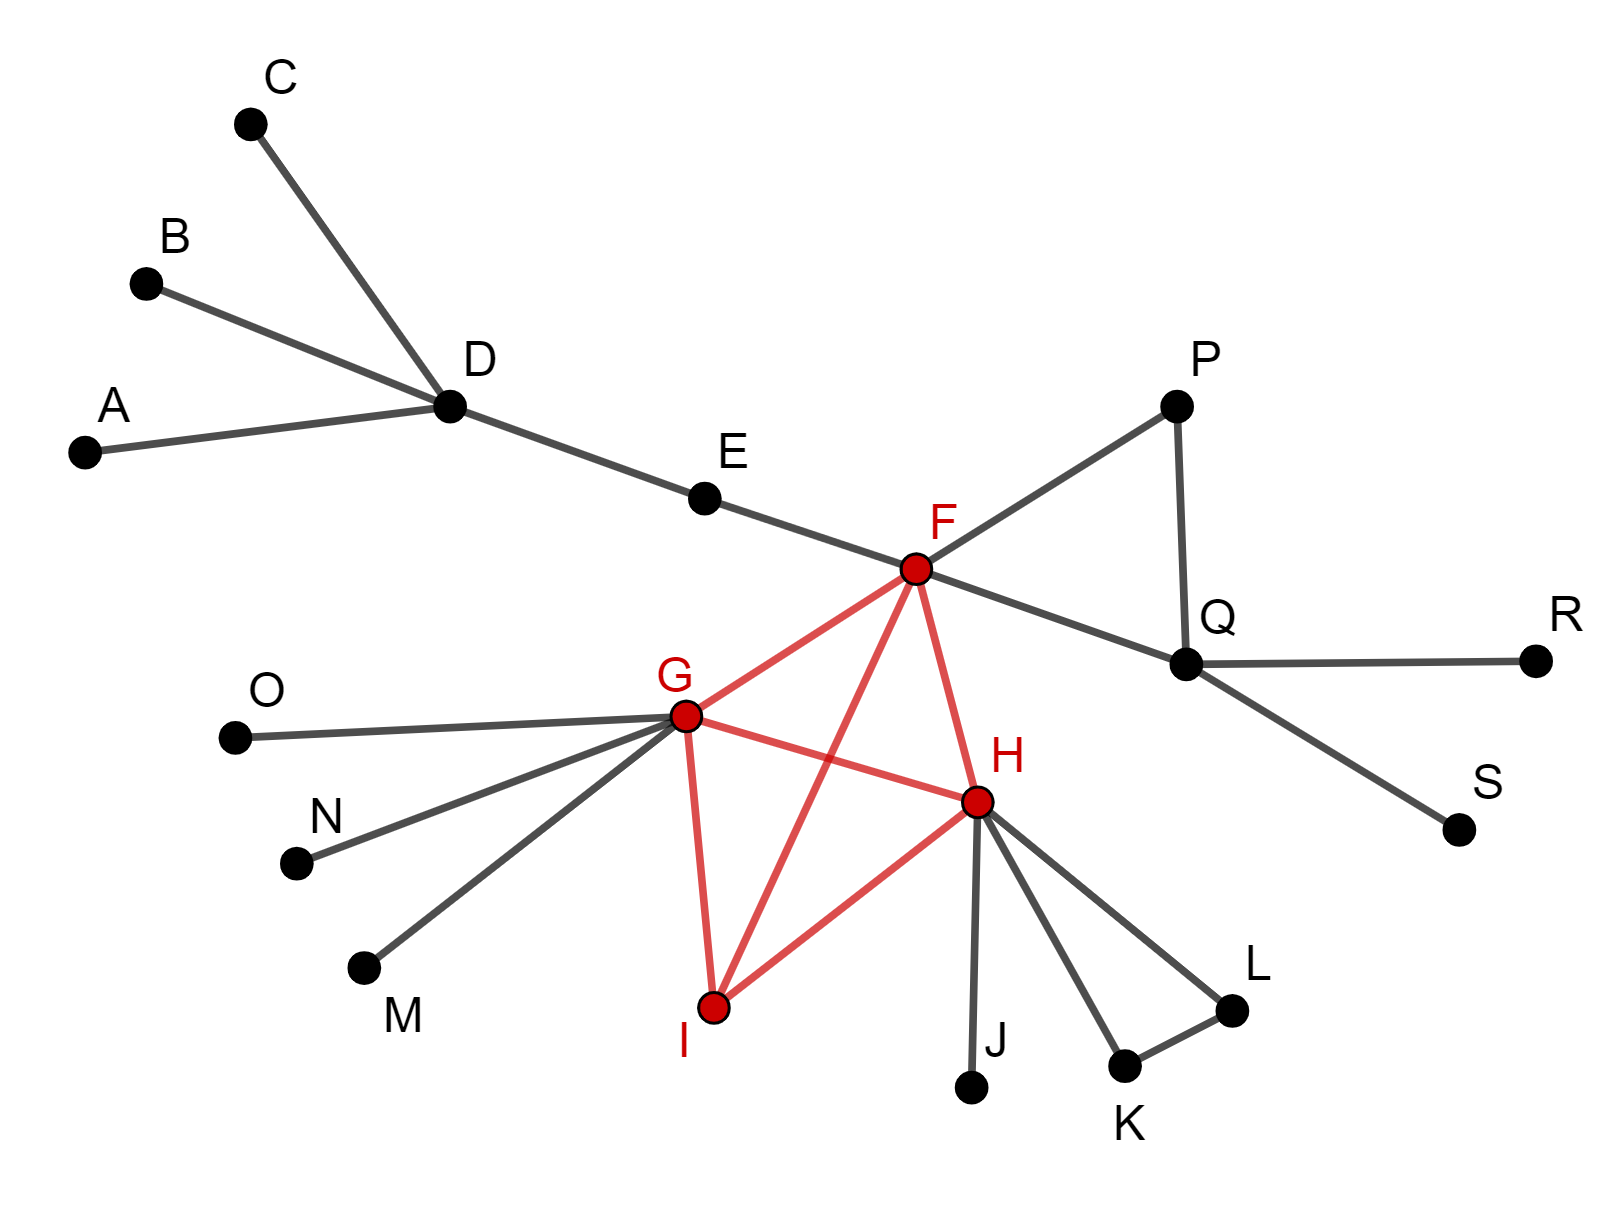
\includegraphics[scale=0.75]{grafo.png}
\end{center}

\textbf{(a) Dê o grau de cada um dos vértices.}\\

\textbf{(b) Qual a soma de todos os graus?} \\

\textbf{(c) Qual o número de arestas?} \\

\textbf{(d) Determine \(\Delta(G)\).} \\

\textbf{(e) Determine \(\delta(G)\).} \\

\textbf{(f) Verifique a desigualdade \(\dfrac{v(G)}{\Delta(G) + 1} \leq \alpha(G) \leq \dfrac{e(G)}{\delta(G)}\) neste grafo \(G\).} \\

\newpage

\begin{center}
\textbf{RESOLUÇÃO}
\end{center}

\textbf{1.} \\

\textbf{(a)}
\begin{enumerate}
\item \(d_G(A) = 1\) 

\item \(d_G(B) = 1\)

\item \(d_G(C) = 1\)

\item \(d_G(D) = 4\)

\item \(d_G(E) = 2\)

\item \(d_G(F) = 6\) 
 
\item \(d_G(G) = 6\)

\item \(d_G(H) = 6\)

\item \(d_G(I) = 3\)

\item \(d_G(J) = 1\)

\item \(d_G(K) = 2\)

\item \(d_G(L) = 2\)

\item \(d_G(M) = 1\)

\item \(d_G(N) = 1\)

\item \(d_G(O) = 1\)

\item \(d_G(P) = 2\)

\item \(d_G(Q) = 4\)

\item \(d_G(R) = 1\)

\item \(d_G(S) = 1\) 
\end{enumerate} 

\textbf{(b)} 

\[\sum \limits_{v \in G} d_G(v) = 1+1+1+4+2+6+6+6+3+1+2+2+1+1+1+2+4
+1 +1= 46\]

\textbf{(c)}

\begin{enumerate}
\item \(AD\)

\item \(BD\)

\item \(CD\)

\item \(DE\)

\item \(EF\)

\item \(FG\)

\item \(FH\)

\item \(FI\)

\item \(FP\)

\item \(FQ\)

\item \(GH\)

\item \(GI\)

\item \(GM\)

\item \(GN\)

\item \(GO\)

\item \(HI\)

\item \(HJ\)

\item \(HK\)

\item \(HL\)

\item \(KL\)

\item \(PQ\)

\item \(QR\)

\item \(QS\)
\end{enumerate}


\textbf{(d)}

Por definição, \(\Delta(G)\) é o maior grau de um vértice de \(G\). Logo, \(\Delta(G) = 6\). \\

\textbf{(e)}

Por definição, \(\delta(G)\) é o menor grau de um vértice de \(G\). Logo, \(\delta(G) = 1\). \\

\textbf{(f)}

Vimos no item (a) que \(G\) tem \(19\) vértices. Logo, \(v(G) = 19\). Já no item (c), vimos que \(G\) tem \(23\) arestas. Logo, \(e(G) = 23\). Resta determinar \(\alpha(G)\). \\

Por definição, \(\alpha(G)\) é o número de elementos do maior conjunto de vértices de \(G\) que são independentes. \\

Recorde que um conjunto \(X\) de vértices de \(G\) é dito independente se para todo vértice \(u, v \in X\), temos que a aresta \(uv\) não é aresta de \(G\).  \\

Argumentaremos que \(\alpha(G)=13\). Para isso, formaremos o maior conjunto de vértices independentes de \(G\). É possível que exista mais de um conjunto com essa propriedade.  \\

Denote por \(X\) o conjunto de vértices de \(G\) independentes que estamos construíndo. Temos que: \(X = \{A, B, C, E, P, R, S, I,  M, N, O, J, K\}\) é um conjunto de vértices de \(G\) independente. Além disso, \(|X| = 13\).  

\begin{center}
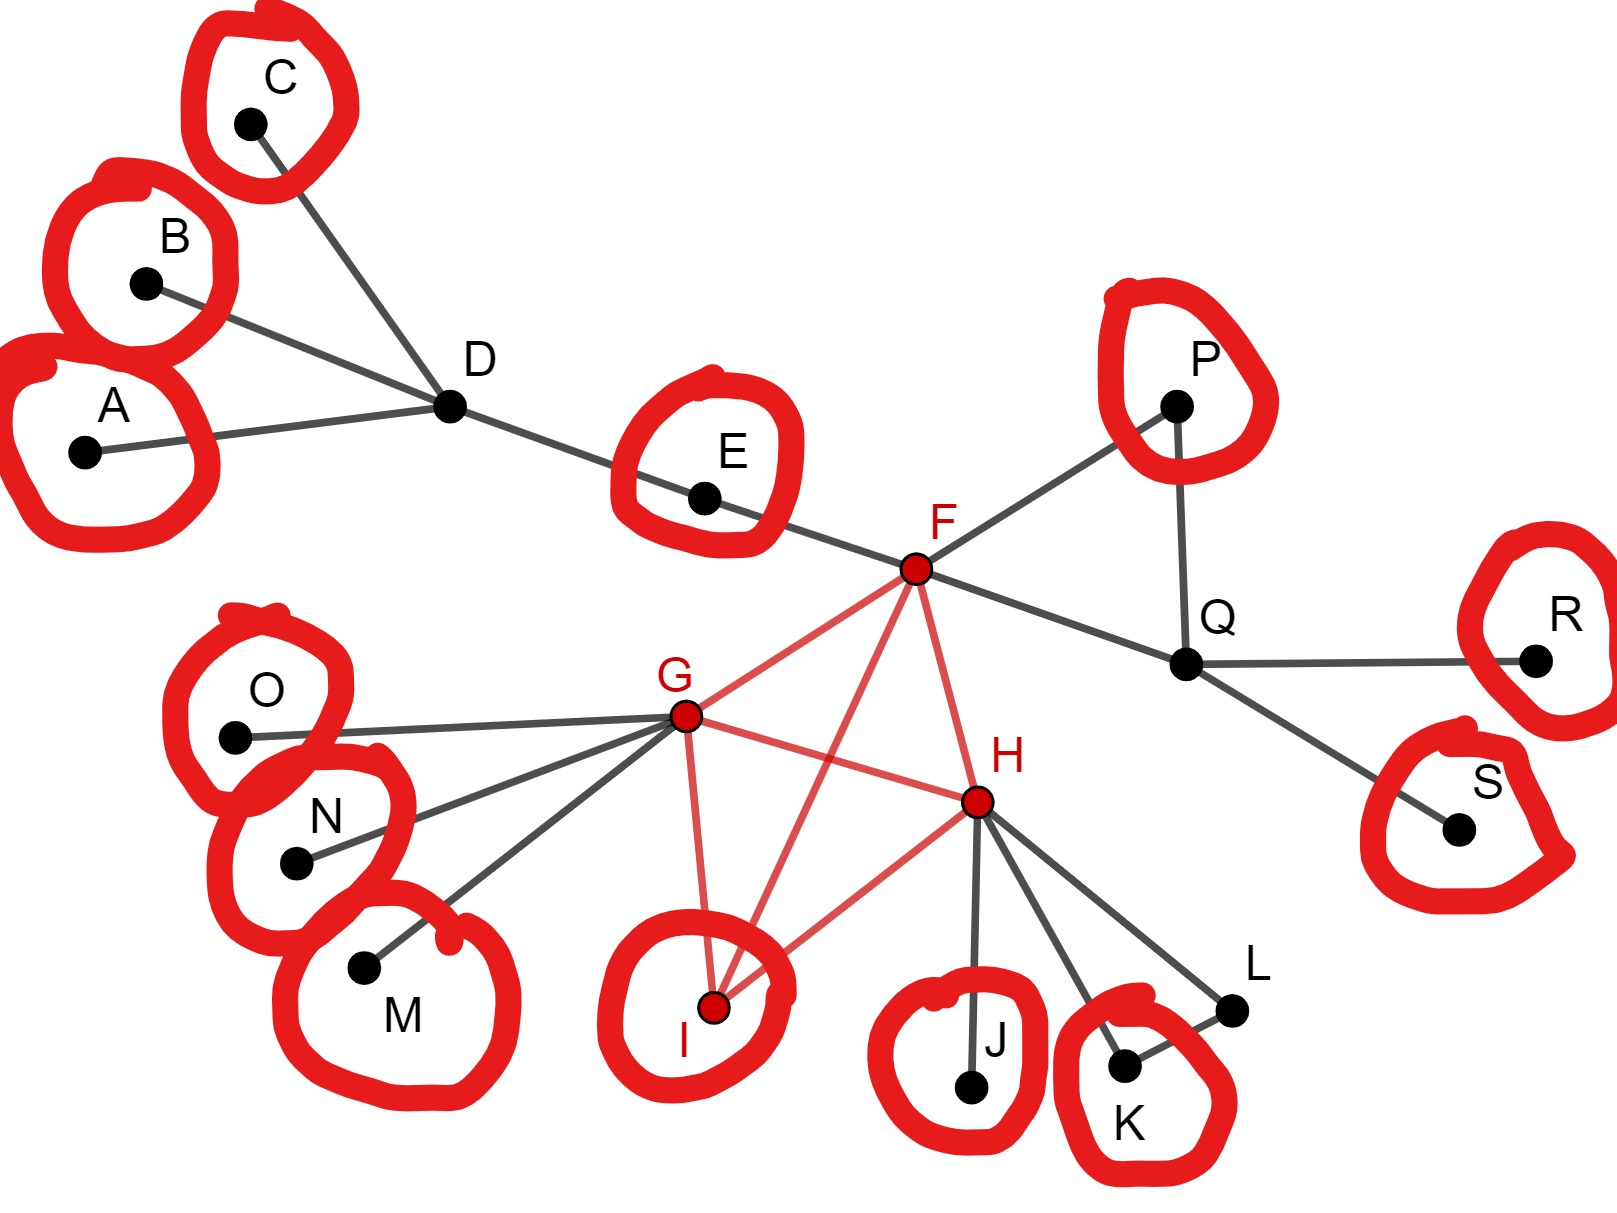
\includegraphics[scale=0.2]{Inkedgrafo.jpg}
\end{center} 

Perceba que o conjunto \(X\) é maximal, pois não existe outro conjunto de vértices independentes \(Y \subset G\) tal que \(X \subset Y\). \\

O grafo \(G\) tem \(19\) vértices. Para qualquer conjunto de vértices independentes \(Y\), temos que ou \(D \in Y\), ou \(D \notin Y\). \\

\begin{center}
Situação 1: \(D \in Y\)
\end{center}

Se \(D \in Y\), então \(A, B, C, E \notin Y\). Assim, \(|Y| \leq 15\) pois há \(19\) vértices e estamos desconsiderando \(4\) para formar \(Y\). Podemos continuar com a investigação: ou \(Q \in Y\), ou \(Q \notin Y\). \\

Se \(Q \in Y\), então \(F, P, R, S \notin Y\). Assim, \(|Y| \leq 11\). Desse modo, \(|Y| < |X|\). Como queremos encontrar \(Y\) tal que \(|X| < |Y|\), então devemos desconsiderar a hipótese de \(Q \in Y\). Portanto, \(Q \notin Y\). De maneira análoga, teremos que \(G \notin Y\) e \(H \notin Y\), pois caso contrário \(|Y| \leq 9\) e \(|Y| \leq 9\) respectivamente. Em ambos, \(|Y| < |X|\). \\  

Recapitulando: se \(D \in Y\), para maximizar a quantidade de elementos de \(Y\), teremos que ter \(Q, G, H \notin Y\). Assim, \(|Y| \leq 12\). Logo, não nunca teremos \(|X| < |Y|\). Se quisermos encontrar um conjunto de vértices independentes maiores do que \(X\), então não podemos ter \(D \in Y\). Assim, ou \( D \notin Y\), ou não existe tal \(Y\). 

\begin{center}
Situação 2: \(D \notin Y\)
\end{center}

Com isso, \(|Y| \leq 18\). Para garantir que não tenhamos \(Y \subset X\), é necessário que \(Y\) possua pelo menos um elemento que não esteja em \(X\). Caso \(Y \subset X\) então \(|Y| \leq |X|\). \\

Assim,  é preciso que \(F \in Y\) ou \(Q \in Y\) ou \(G \in Y\) ou \(H \in Y\) ou \(L \in Y\).  \\

Se \(F \in Y\), então \(E, P, Q, G, I, H \notin Y\). Logo, \(|Y| \leq 12\). Desse modo, \(|Y| <|X|\). Assim, não podemos ter \(F \in Y\). Portanto, \(F \notin Y\). Daí, \(|Y| \leq 17\).\\

Se \(Q \in Y\), então \(P, R, S \notin Y\). Logo, \(|Y| \leq 14\). Note que \(G \notin Y\) (caso contrário \(|Y| \leq 9\)). Daí teremos que \(|Y| \leq 13 = |X|\). Assim, podemos desconsiderar o caso em que \(Q \in Y\). Desse modo, \(|Y| \leq 16\), já que \(D, F, G \notin Y\). \\

Se \(G \in Y\), então \(O, M, N, I \notin Y\). Assim, \(|Y| \leq 12\). Ou seja, \(|Y| < |X|\). Portanto, não podemos ter \(G \in Y\). Daí, \(G \notin Y\) e \(|Y| \leq 15\). \\

Analogamente, se \(H \in Y\), teremos que \(|Y| \leq 11\) (Por quê?). Assim, \(H \notin Y\) e \(|Y| \leq 14\). Porém, só sobra o caso em que \(L \in Y\), que implica que \(K \notin Y\). Daí, \(|Y| \leq 13 = |X|\). \\

Logo, não nunca teremos \(|X| < |Y|\). Então, concluí-se que não existe um conjunto de vértices independentes \(Y \subset G\) tal que \(|X| < |Y|\). Portanto, por definição, \[\alpha(G) = |X| = 13\]  
 
Com isso, temos que:

\begin{itemize}
\item \(\dfrac{v(G)}{\Delta(G)+1}= \dfrac{19}{6+1}=\dfrac{19}{7} < \dfrac{21}{7} = 3\)

\item \(\alpha(G)=13\)

\item \(\dfrac{e(G)}{\delta(G)}=\dfrac{23}{1}=23\)
\end{itemize}

Assim, \[\dfrac{v(G)}{\Delta(G) + 1} \leq \alpha(G) \leq \dfrac{e(G)}{\delta(G)}\] Pois, 
\[\dfrac{19}{7} \leq 13 \leq 23\]

\end{document}